% YOLO-FastestV2 Architecture Diagram — TikZ for LaTeX
% Compile: pdflatex or xelatex
% Requires: \usepackage{tikz} \usetikzlibrary{shapes,arrows,positioning,fit,backgrounds}
\documentclass[tikz,border=5pt]{standalone}
\usepackage{tikz}
\usetikzlibrary{shapes.geometric, arrows, positioning, fit, backgrounds, calc}
\usepackage{xcolor}

\begin{document}
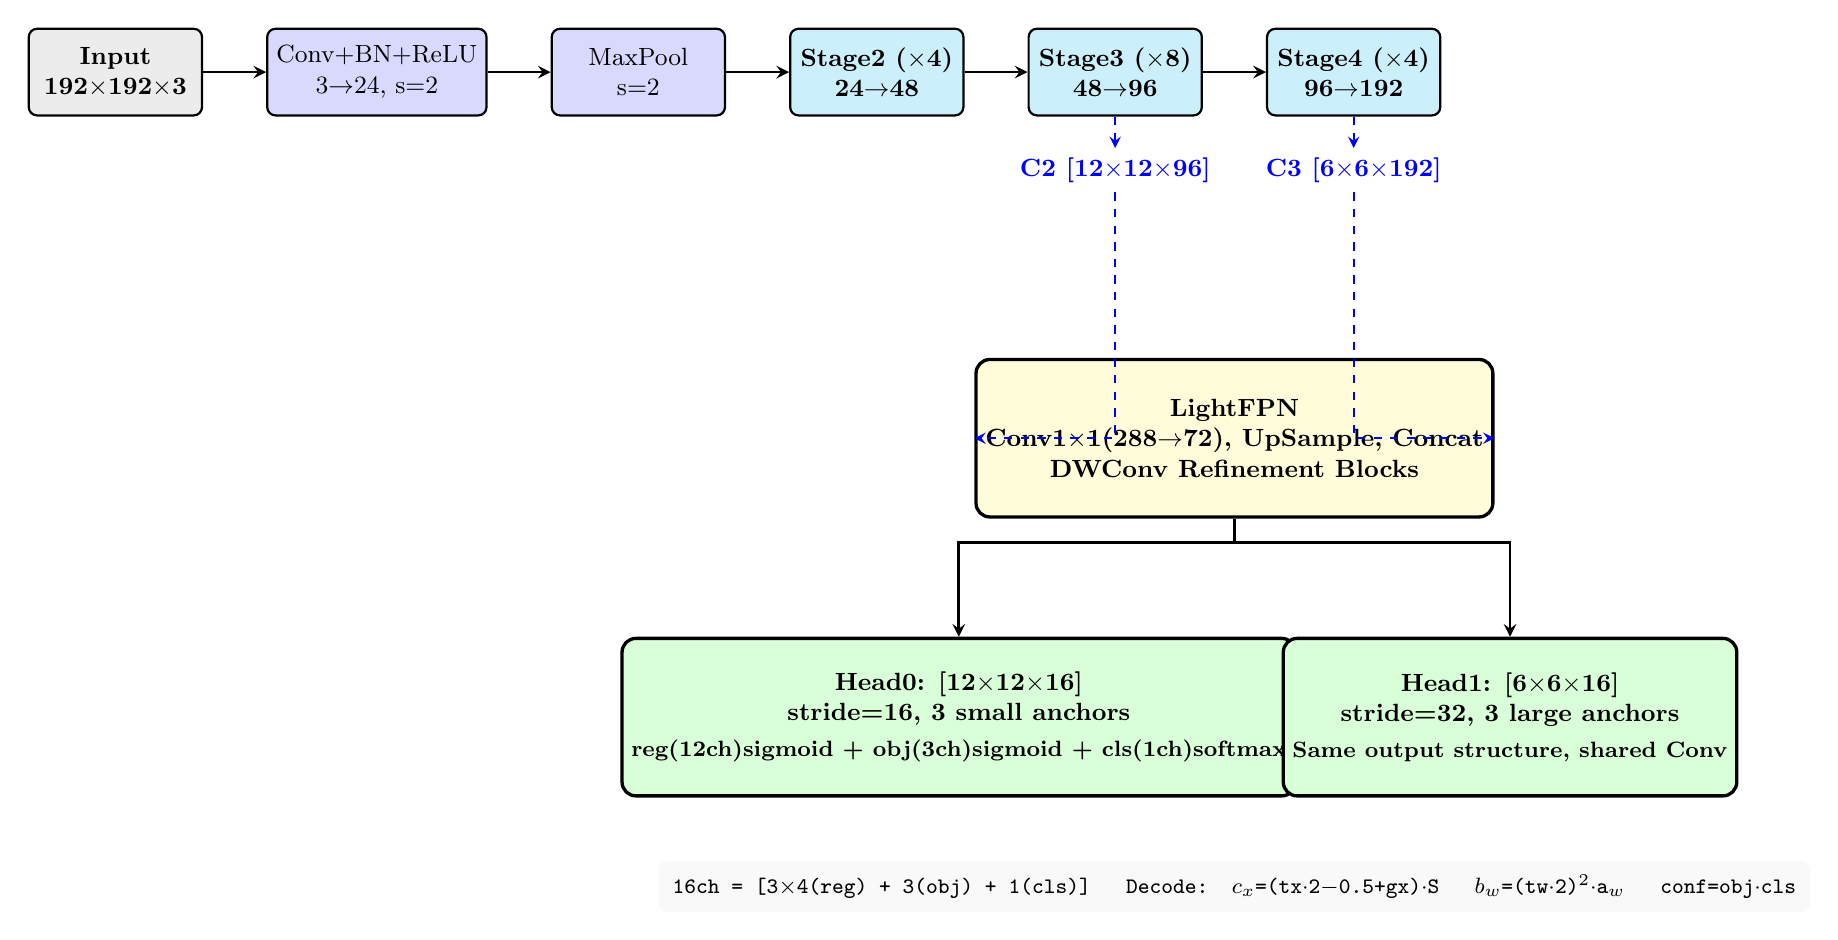
\begin{tikzpicture}[
    box/.style={rectangle, rounded corners=3pt, draw=black, line width=0.8pt,
                minimum width=2.2cm, minimum height=1.1cm, align=center, font=\small},
    bigbox/.style={rectangle, rounded corners=5pt, draw=black, line width=1.2pt,
                   minimum width=5.5cm, minimum height=2.0cm, align=center, font=\small\bfseries},
    arrow/.style={->, >=stealth, line width=1pt},
    dasharrow/.style={->, >=stealth, dashed, line width=0.8pt, blue}
]

% === BACKBONE ===
\node[box, fill=gray!15, font=\small\bfseries] (input) {Input\\192$\times$192$\times$3};
\node[box, fill=blue!15, right=0.8cm of input] (conv1) {Conv+BN+ReLU\\3$\to$24, s=2};
\node[box, fill=blue!15, right=0.8cm of conv1] (pool) {MaxPool\\s=2};
\node[box, fill=cyan!20, right=0.8cm of pool, font=\small\bfseries] (s2) {Stage2 ($\times$4)\\24$\to$48};
\node[box, fill=cyan!20, right=0.8cm of s2, font=\small\bfseries] (s3) {Stage3 ($\times$8)\\48$\to$96};
\node[box, fill=cyan!20, right=0.8cm of s3, font=\small\bfseries] (s4) {Stage4 ($\times$4)\\96$\to$192};

\draw[arrow] (input) -- (conv1);
\draw[arrow] (conv1) -- (pool);
\draw[arrow] (pool) -- (s2);
\draw[arrow] (s2) -- (s3);
\draw[arrow] (s3) -- (s4);

% C2, C3 labels
\node[below=0.4cm of s3, font=\small\bfseries, blue] (c2) {C2 [12$\times$12$\times$96]};
\node[below=0.4cm of s4, font=\small\bfseries, blue] (c3) {C3 [6$\times$6$\times$192]};
\draw[dasharrow] (s3.south) -- (c2.north);
\draw[dasharrow] (s4.south) -- (c3.north);

% === FPN ===
\node[bigbox, fill=yellow!15, below=1.8cm of $(c2.south)!0.5!(c3.south)$, yshift=-0.3cm] (fpn)
    {LightFPN\\Conv1$\times$1(288$\to$72), UpSample, Concat\\DWConv Refinement Blocks};

\draw[dasharrow] (c2.south) |- (fpn.west);
\draw[dasharrow] (c3.south) |- (fpn.east);

% === HEADS ===
\node[bigbox, fill=green!15, below=1.5cm of fpn, xshift=-3.5cm] (head0)
    {Head0: [12$\times$12$\times$16]\\stride=16, 3 small anchors\\[2pt]
     \footnotesize reg(12ch)sigmoid + obj(3ch)sigmoid + cls(1ch)softmax};
\node[bigbox, fill=green!15, below=1.5cm of fpn, xshift=3.5cm] (head1)
    {Head1: [6$\times$6$\times$16]\\stride=32, 3 large anchors\\[2pt]
     \footnotesize Same output structure, shared Conv};

\draw[arrow] (fpn.south) -- ++(0,-0.3) -| (head0.north);
\draw[arrow] (fpn.south) -- ++(0,-0.3) -| (head1.north);

% === CHANNEL DETAIL ===
\node[below=0.8cm of $(head0.south)!0.5!(head1.south)$, font=\footnotesize\ttfamily,
      fill=gray!5, rounded corners=3pt, inner sep=5pt] {
    16ch = [3$\times$4(reg) + 3(obj) + 1(cls)] \quad
    Decode: $c_x$=(tx$\cdot$2$-$0.5+gx)$\cdot$S \quad
    $b_w$=(tw$\cdot$2)$^2$$\cdot$a$_w$ \quad conf=obj$\cdot$cls
};

\end{tikzpicture}
\end{document}
